\documentclass[14pt]{extreport}
\usepackage{gost}

%Тут можно вставить дополнительные пакеты

\begin{document}
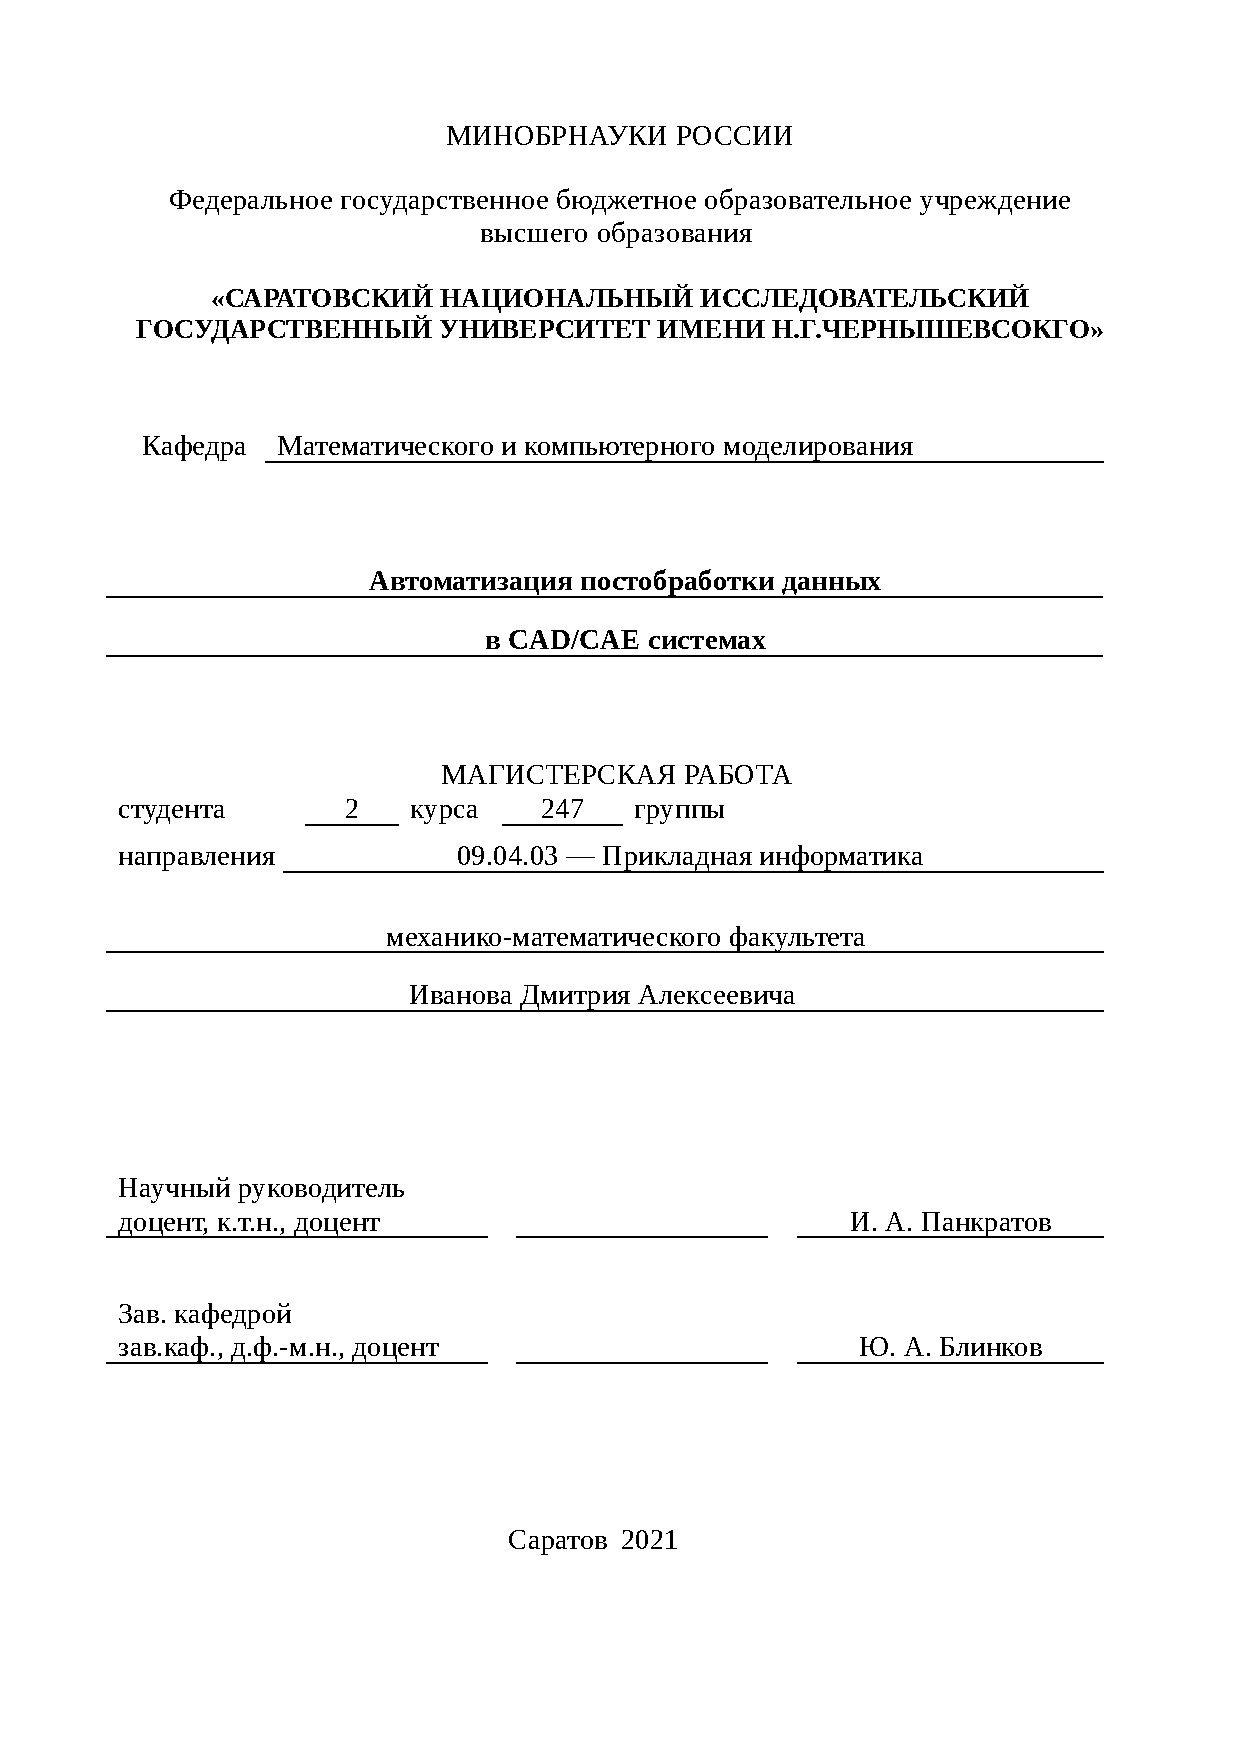
\includepdf[pages={1}]{titulCourse.pdf}
% \includepdf[pages={1}]{titulDiplom.pdf}

\tableofcontents

\intro
Введение должно включать:
\begin{itemize}
\item общую информацию о состоянии разработок по выбранной теме;  
\item обоснование актуальности и новизны темы, связь данной работы с другими научно-исследовательскими работами;
\item цель работы и решаемые задачи. 
\end{itemize}
% Введение начинается с нового листа.

%\chapter{Основная часть\label{chapter2}}%


\conclusions

% Оформляем библиографию в соответствии с ГОСТ 7.0.5
\bibliographystyle{ugost2008}
% если хотим включить все источники из библиографии даже не имеющие ссылки из текта
\nocite{*}
% файл с библиографией
\bibliography{biblio.bib}

\Appendix % Приложения

\end{document}
